\documentclass[a4paper, 12pt]{report}

% Packages
\usepackage[utf8]{inputenc}
\usepackage{graphicx}
\usepackage{float}
\usepackage{hyperref}
\usepackage{fancyhdr}
\usepackage{titlesec}
\usepackage{lipsum}
\usepackage{amsmath}
\usepackage{biblatex}
\usepackage{minted}
\usepackage[a4paper, margin=1in]{geometry}
\addbibresource{bibliography.bib}

% Mise en page
\pagestyle{fancy}
\fancyhf{}
\setlength{\headheight}{15pt}
\renewcommand{\headrulewidth}{0.5pt}
\renewcommand{\footrulewidth}{0pt}
\lhead{\leftmark}
\rhead{\thepage}
\renewcommand{\chaptermark}[1]{\markboth{\MakeUppercase{#1}}{}}
\titleformat{\chapter}[display]{\normalfont\huge\bfseries}{\chaptertitlename\ \thechapter}{20pt}{\Huge}
\graphicspath{ {./images/} }

\begin{document}

% Page de garde
\begin{titlepage}
    \centering{
        % Nom de la matière
        \textbf{Deepening and opening project}
        \noindent\rule{\textwidth}{0.4pt}
        \vfill
        % Nom du rapport
        \Huge
        Project report\\
        Evidential mapping for mobile robots\\
        \normalsize
        \vfill
        \textbf{Réalisé par :}\\
        % Nom des auteurs
        \normalsize
        Alix ANNERAUD\\
        Dimitri TIMOZ\\
        
        \vspace{1cm}

        \textbf{Supervised by:}\\
        Hind LAGHMARA HACHEMI\\
        \normalsize
        \vspace{1cm}
        Academic year 2023-2024\\
        \vspace{1cm}
        
\includegraphics[width=200px]{images/INSA.jpg}
    }
\end{titlepage}

% Table des matières
\tableofcontents

\newcommand{\todo}{\begin{center}\Huge A faire\normalsize \end{center}} % A supprimer lorsque le rapport sera terminé
\chapter*{Abstract}

In this project, we implement an evidential mapping approach using the Dempster-Shafer theory of evidence, a mathematical framework that allows for reasoning under uncertainty and combining evidence from multiple sources. Central to our implementation is the concept of the belief mass function, which serves as a mathematical representation of uncertainty within a given frame of discernment. This framework is particularly promising for multi-agent systems, where the integration and analysis of disparate evidence from various agents can enhance decision-making processes. Our approach applies these theories to optimize the performance of mobile robots in dynamic environments, employing advanced computational techniques such as parallelization and vectorization to improve efficiency. The potential for scaling this model to multi-agent scenarios offers significant opportunities for advancements in distributed robotic systems.

\chapter{Theory}

\section{Introduction}

Our project is primarily based on the Dempster-Shafer theory of evidence
(see articles \cite{2.5D_Evidential_Grids_for_Dynamic_Object_Detection} and \cite{Cloud_Update_of_Tiled_Evidential_Occupancy_Grid_Maps_for_the_Multi_Vehicle_Mapping})
, which is a mathematical framework for reasoning under uncertainty and combining evidence from multiple sources.


\section{Belief Mass Function}

In the Dempster-Shafer theory of evidence, a fundamental concept is that of the belief mass function.
It serves as a mathematical representation of uncertainty associated with propositions within a given frame of discernment.

\subsection{Definition}

The belief mass function $ m $ assigns a numerical value to each subset of the frame of discernment, indicating the degree of belief or support for that subset. Formally, for a frame of discernment $ \Omega $, the belief mass function is defined as:

$$ m: 2^\Omega \rightarrow [0,1] $$

Where:

\begin{itemize}
    \item $ 2^\Omega $ denotes the power set of $ \Omega $, representing all possible subsets of $ \Omega $.
    \item $ m(A) $ represents the belief mass assigned to subset $ A \subseteq \Omega $.
\end{itemize}

In our case of an evidential grid, the frame of discernment is $\Omega = \{F, O, \Omega, \emptyset\}$, where:

\begin{itemize}
    \item $ F $ represents the proposition of unoccupied space.
    \item $ O $ represents the proposition of occupied space.
    \item $ \Omega $ denotes the entire frame of discernment (all possible propositions).
    \item $ \emptyset $ denotes the empty set, representing ignorance or lack of information.
\end{itemize}

In summary, belief mass functions provide a formalism for representing and reasoning with uncertain evidence, making them a key component of the Dempster-Shafer theory and applications such as decision-making under uncertainty and information fusion.


\subsection{Properties}

\begin{itemize}
    \item Normalization: The sum of belief masses assigned to all subsets of $ \Omega $ equals 1:
          $$ \sum_{A \subseteq \Omega} m(A) = 1 $$
    \item Conflict Measure: The belief mass function accounts for conflicts or overlaps between different subsets. This is crucial for combining evidence from multiple sources.
    \item Ignorance Representation : The belief mass function can explicitly model ignorance or lack of information by assigning mass to the empty set $\emptyset$.
          This represents the uncertainty about all subsets of $ \Omega $.
\end{itemize}

\subsection{Interpretation}

\begin{itemize}
    \item Support: High belief mass assigned to a subset indicates strong support or evidence for the propositions within that subset.
    \item Uncertainty: Low belief mass suggests uncertainty or lack of evidence for the propositions in the subset.
\end{itemize}



\section{Dempster-Shafer theory} \label{sec:dempster_shafer_theory}

The Dempster combination of evidential theory is a data fusion technique used within the framework of evidence theory, also known as Dempster-Shafer theory.
This theory was developed by Glenn Shafer and Arthur P. Dempster in the 1960s and 1970s.
Evidence theory is an approach to managing uncertainty and fusing information sources that may contain uncertainties or contradictions.
It differs from classical probability theory in that it allows for more flexible treatment of uncertainty, including modeling ignorance and conflict.

The Dempster combination is a fusion operation that combines belief functions (or mass functions) from different information sources to produce a global belief function.
This operation is based on Dempster's combination rules, which take into account the degrees of concordance and discordance among different information sources:

$$
    \forall A \subseteq \Omega, m_{1\cap2}(A) = \sum_{B\cap A = A | C, C \subseteq \Omega} m_{1}(B) \times m_{2}(C)
$$

$$
    m_{1\oplus2}(A) = \frac{m_{1\cap2}(A)}{1-m_{1\cap2}(\emptyset)}, \forall A\subseteq \Omega, A \neq \emptyset
$$

$$
    m_{1 \oplus 2}(\emptyset) = 0
$$

In our case of an evidential grid, the frame of discernment is $\Omega = \{F, O, \Omega, \emptyset\}$, which translates to the following combination rules:

$$
    \begin{cases}
        m_{1\cap2}(F) = \frac{m_{1}(\Omega) \times m_{2}(F) + m_{1}(F) \times m_{2}(\Omega) + m_{1}(F) \times m_{2}(F)}{1 - K} \\
        m_{1\cap2}(O) = \frac{m_{1}(\Omega) \times m_{2}(O) + m_{1}(O) \times m_{2}(\Omega) + m_{1}(O) \times m_{2}(O)}{1 - K} \\
        m_{1\cap2}(\Omega) = \frac{m_{1}(\Omega) \times m_{2}(\Omega)}{1 - K}                                                  \\
        m_{1\cap2}(\emptyset) = 0
    \end{cases}
$$

With the level of conflict measured by:

$$
    K = m_{1}(F) \times m_{2}(O) + m_{1}(O) \times m_{2}(F)
$$

In summary, the Dempster Combination of Evidential Theory is a method for merging different uncertain information sources within the evidence theory framework, using Dempster's combination rules to produce a more robust overall estimate.



\section{Age consideration} \label{sec:age_consideration}

In the context of updating belief functions to account for the temporal aspect, an age consideration is introduced. This accounts for the change in information over time, allowing for the adjustment of belief functions based on the age of the data.

The adjustment factor, denoted as $ \alpha $, is determined by the difference in time between the old and new observations, normalized by a time constant $ \tau $. This factor reflects the degree of confidence attributed to the new observation relative to the old one.

$$
    \alpha = e^{\frac{t_{old}-t_{new}}{\tau}}
$$

Where:
\begin{itemize}
    \item $ t_{old} $ represents the timestamp of the old observation.
    \item $ t_{new} $ represents the timestamp of the new observation.
    \item $ \tau $ is a time constant determining the rate of decay of belief in older observations.
\end{itemize}

Upon incorporating the age consideration, the updated belief functions for focal elements (e.g., propositions) $F$ (support), $O$ (opposition), and $\Omega$ (the entire frame of discernment) at time $ t_{\text{new}} $ are calculated as follows:

$$
    \begin{cases}
        m_{G\{i,j\},t_{new}}^{\alpha}(F) = \alpha \times m_{G\{i,j\},t_{old}}(F) \\
        m_{G\{i,j\},t_{new}}^{\alpha}(O) = \alpha \times m_{G\{i,j\},t_{old}}(O) \\
        m_{G\{i, j\}, t_{new}}^{\alpha}(\Omega) = (1 - \alpha) + \alpha \times m_{G\{i, j\}, t_{old}}(\Omega)
    \end{cases}
$$


Where:
\begin{itemize}
    \item $m_{G\{i,j\},t}$ denotes the belief function associated with the focal element $ G\{i,j\} $ at time $ t $.
    \item The superscript $\alpha$ indicates the updated belief function after considering the age factor.
\end{itemize}


This adjustment allows for the integration of temporal dynamics into the Dempster Combination of Evidential Theory, enabling the refinement of belief functions based on the recency and relevance of information.

\section{Pignistic probability} \label{sec:pignistic_probability}

In the Dempster-Shafer theory, pignistic probabilities offer a way to derive a single probability distribution from the belief mass function.
This transformation from belief masses to probabilities facilitates decision-making and inference in a manner akin to classical probability theory.

\subsection{Definition}

Pignistic probability, denoted as $ Bel $, assigns a probability value to each individual element of the frame of discernment $ \Omega $. It represents the degree of belief that a specific proposition within $ \Omega $ is true.

$$ Bel: \Omega \rightarrow [0,1] $$

Where $ Bel(A) $ denotes the pignistic probability assigned to proposition $ A \in \Omega $.

\subsection{Computation}

Pignistic probability is computed using the belief mass function $ m $ and the concept of the focal elements, which are the non-empty subsets of $ \Omega $. For a focal element $ A $, the pignistic probability is calculated as the sum of belief masses of all subsets containing $ A $, normalized by the total belief mass assigned to all focal elements:

$$ Bel(A) = \sum_{B \in F(A)} \frac{m(B)}{1 - m(\emptyset)} $$

Where:
\begin{itemize}
    \item $ F(A) $ represents the set of all focal elements containing proposition $ A $.
    \item $ m(\emptyset) $ is the belief mass assigned to the empty set, representing the total ignorance.
\end{itemize}

\subsection{ Interpretation }

Pignistic probabilities offer a probabilistic interpretation of belief masses, providing a means to quantify uncertainty and make decisions based on the available evidence. Unlike belief masses, which assign support to subsets of $ \Omega $, pignistic probabilities assign probabilities directly to individual propositions within $ \Omega $.

\chapter{Practical application}    

\section{Introduction}

\section{Software features}

\subsection{Overview}

The software developed for this project is a ROS node that implements the algorithms described in the previous sections.
The node subscribes to the \texttt{laserScan} topic to receive laser data from the robot's LIDAR sensor and the \texttt{odometry} topic to receive odometry data from the robots.

\subsection{The map}

The map is represented as a 2D grid of cells, where each cell contains a belief mass function and last update timestamp.
The map is initialized with a uniform belief mass function where the mass of the unknown state is $1$ and the other states have mass $0$.


\subsection{Laser scan to grid conversion}

The node receives laser scan data from the robot's LIDAR sensor and converts it into a 2D grid representation.
For each laser scan, we create a new grid with the dimensions of the laser's field of view and resolution.
For each ray, we draw a line from the robot's position to the end point of the ray and update the belief mass function by setting the masse of the free state to an estimation of the captor's accuracy.
Once the ray reaches an obstacle, we set the mass of the occupied state to the same value as the free state when a cell is considered free.
Then, we have an local EOGM.

\subsection*{Map fusion}

Once the local EOGM is computed, we fuse it with the global EOGM.
Just before the fusion, we update the global EOGM by decreasing the mass of the oldest cells which could be affected by the new local EOGM.
Then, we fuse the local EOGM with the global EOGM using the Dempster's rule of combination.



\section{Optimization}

\subsection{Introduction}

Since our algorithm is computationally intensive and is intended to be used in real-time applications, it is essential to optimize its performance.
In this section, we discuss the optimization techniques employed to enhance the efficiency of our implementation.

\subsection{Parallelization}

One of the most effective ways to improve the performance of our algorithm is to parallelize the computation.
Since OpenMP is integrated with ROS, we can utilize its parallel programming capabilities to distribute the computation across multiple CPU cores.
However, we need to be careful when parallelizing the computation since concurrent access to shared data structures can lead to memory consistency issues.
To avoid such problems, OpenMP provides the \texttt{\#pragma omp critical} macro to specify critical sections that should be executed atomically by a single thread.
On the Robotnik Summit-XL HL, the processor is a 9th generation Intel processor (Coffee Lake Refresh) with 6 cores and 12 threads, this should allow from a 6x to 12x performance improvement for operations that can be parallelized.
We applied parallelization to the computation of the following parts of our algorithm:
\begin{itemize}
    \item Laser scan to grid conversion
    \item Belief mass function fusion
    \item Pignistic probability computation
    \item Age consideration computation
\end{itemize}

\subsection{Vectorization}

In a similar fashion to parallelization, vectorization is another optimization technique that can significantly enhance the performance of our algorithm.
This can be achieved by utilizing SIMD (Single Instruction, Multiple Data) instructions provided by modern processors to perform operations on multiple data elements simultaneously.
On the Robotnik Summit-XL HL, the processor is a 9th generation Intel processor (Coffee Lake Refresh) with AVX2 support, allowing for efficient vectorization of operations.
This allowed perform 8 32 bit floating point operations in parallel using AVX2 instructions.
This should allow a performance improvement of up to 8x for operations that can be vectorized.
In our case, we used vectorization to optimize the following parts of our algorithm:
\begin{itemize}
    \item Belief mass function fusion
    \item Pignistic probability computation
    \item Age consideration computation
\end{itemize}

\subsection{Memory optimization}

Memory optimization is another crucial aspect of performance enhancement.
By reducing the memory footprint of our algorithm, we can minimize the number of dynamic memory allocations and deallocations, which can significantly impact performance due to the overhead of dynamic memory management and system calls.
Here are some memory optimization techniques we used in our implementation:

\begin{itemize}
    \item Fixed-size arrays: Using fixed-size arrays instead of dynamic arrays can reduce the overhead of dynamic memory management and improve cache locality.
          For example, we can use the `std::vector::reserve` and  `std::vector::resize` functions to resize the vector without reallocation.
    \item Stack memory: Using stack memory instead of heap memory for temporary variables can reduce the overhead of dynamic memory management.
    \item Reference passing: Passing variables, especially large data structures,by reference instead of by value can reduce the overhead of copying large data structures.
\end{itemize}





\chapter{Manual}

This chapter provides a guide for building, running, and using the project.
The project is a ROS package designed to fuse multiple maps into a single evidential occupancy grid map.
It consists of a single node that subscribes to odometry and LIDAR data and publishes the fused map.
The provided commands are intended to be run with the bourne shell on a Debian-based system.

\section{Build}

\subsection{Prerequisites}

First of all, you will need the following software installed:
\begin{itemize}
    \item \textbf{ROS Melodic} : You can install it by following the instructions on the official website: \url{http://wiki.ros.org/melodic/Installation}. You likely need a Ubuntu 18.04 (Bionic Beaver) system.
    \item \textbf{Octomap} : Check the package page on the ROS wiki for installation instructions: \url{http://wiki.ros.org/octomap}.
\end{itemize}

\subsection{Build}

Clone the repository from GitHub:
\begin{minted}{bash}
git clone https://github.com/DimitriTimoz/tiled-evidential-occupancy-grid
\end{minted}

To build the project, run the following commands in the root directory of the project:
\begin{minted}{bash}
catkin_make install
\end{minted}

\section{Documentation}

The documentation of the project can be generated using the following command in the root directory of the project:

\begin{minted}{bash}
source devel/setup.bash
doxygen Doxyfile
\end{minted}

\section{Run}

After starting the ROS master (with the command \texttt{roscore}), you can run the project with the following commands in the root directory of the project

\begin{minted}{bash}
source devel/setup.bash
sh scripts/run.sh
\end{minted}

or :

\begin{minted}{bash}
source devel/setup.bash
rosrun map_fusion map_fusion_node
\end{minted}

\section{Use}

\subsection{Set the parameters}

The project's parameters can be configured in the \texttt{src/map\_fusion\_node.cpp} file.
In the constructor of the \texttt{EvidentialGrid} class, you can set the following parameters:

\begin{itemize}
\item \texttt{Map size}: width, height
\item \texttt{Resolution}: the map's resolution in meters per cell
\item \texttt{ODOM topic}: the topic where odometry data is published
\item \texttt{LIDAR topic}: the topic where LIDAR laser scan data is published
\end{itemize}

\subsection{Visualize}

To visualize the generated map, you can use the \texttt{rviz} tool. Once \texttt{rviz} is started, just add a \texttt{ColorOccupancyGrid} and set the following properties:

\begin{itemize}
    \item \texttt{Topic} : \texttt{/global\_eogm}
    \item \texttt{Voxel coloring Scheme} : \texttt{Cell color}
\end{itemize}

It is recommanded to enable graphics acceleration / GPU passthrough if you run your system in a virtual machine.
\chapter{Results and future work}

\section{Experimental results}

To evaluate the proposed method, we conducted experiments using the \textit{SummitXL} robot by \textit{Robotnik}, which is equipped with a laser scanner and IMU sensors. The test environment was a room measuring approximately $7 \times 6$ meters. We moved the robot slowly to minimize noise in the data collected by the IMU.

\begin{figure}[H]
    \centering
    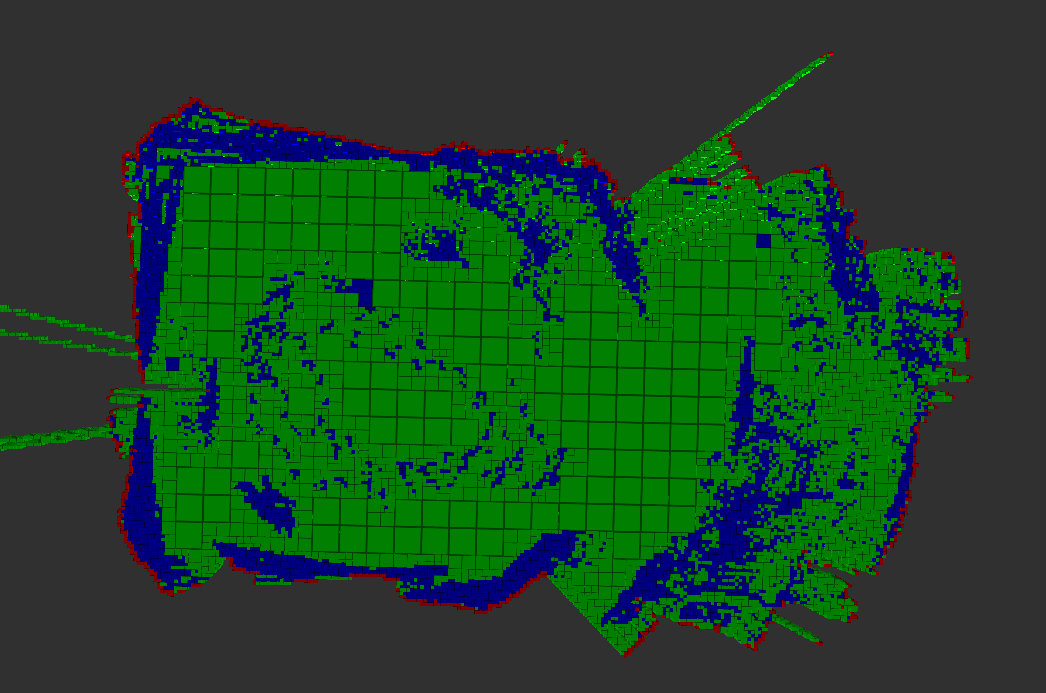
\includegraphics[width=\textwidth]{images/top_screenshot.png}
    \caption{Top view of the octomap generated by our program in the P.E.R.M.I.S. environment. The gray area represents unknown space, the green area represents free space, and the red area represents occupied space. Only the major probability values are shown.}
\end{figure}

In the P.E.R.M.I.S. environment, using the \textit{SummitXL} robot, we obtained the following results:

\begin{itemize}
    \item The octomap provides a coherent representation of the environment, with the boundaries of the room clearly defined.
    \item Moving objects are detected; in the figure, the circle made of blue points represents a person moving around.
    \item Near the room boundaries, the program detects numerous conflicts, likely due to the robot's movement and IMU imperfections.
    \item Attenuation could be useful for detecting moving objects. Occupied cells surrounded by conflict cells often indicate a fixed object, whereas disappearing conflicts usually indicate a moving object.
    \item The program runs in real-time at approximately 15 Hz and could be significantly improved by reducing the resolution.
\end{itemize}

\section{Future work}

The proposed implementation is a first step towards using Evidential Grids for detecting moving objects.
However, several improvements are needed to enhance its efficiency and reliability.

\subsection{Implementation improvements}

Here are the main improvements that could be made to the implementation:

\begin{itemize}
    \item \textbf{GPU acceleration}: The program could be further optimized for faster performance by using GPUs.
    \item \textbf{Standardization of ROS messages}: The lack of standardization in ROS messages is problematic, as different robot manufacturers do not use the laser scan message uniformly.
          This has prevented us from implementing a robust system to filter reliable data.
    \item \textbf{Suitable message for EOGM data}: Despite the existing \texttt{Octomap} message, it is not ideal for further processing of EOGM data.
          One solution could be to use an existing message for RViz and another standardized message for other nodes.
          However, this would sacrifice the size optimization of the \texttt{Octomap} message, leading to slower communication.
          Another solution could be to develop a new message with its own RViz plugin, though this would require significant effort.
\end{itemize}

\subsection{Methodological improvements}

Methodologically, the IMU data exhibits significant noise due to the robot's movements, leading to wide conflict areas, especially near room boundaries.
One potential solution could involve upgrading to a more accurate IMU or implementing methods to mitigate conflicts near fixed objects.
Incorporating SLAM algorithms may enhance robot localization and reduce conflicts.
Additionally, leveraging the robot's movement could aid in detecting moving objects.
For instance, observing the disappearance of conflicts when the robot moves forward could indicate the presence of a moving object.
Furthermore, analyzing the robot's movement patterns could contribute to refining localization accuracy and orientation estimation.

\chapter{Conclusion}

\section*{Conclusion}

In this project, we successfully implemented an evidential mapping approach using the Dempster-Shafer theory of evidence to enhance the performance of mobile robots in dynamic environments. Our experimental results demonstrated the capability of our system to create coherent representations of the environment, detect moving objects, and operate in real-time.

The use of the \textit{SummitXL} robot in a controlled environment allowed us to validate the effectiveness of our method. We were able to generate accurate octomaps that defined the boundaries of the room and detect moving objects. Despite the noise in the IMU data, the program managed to perform reliably, although there is room for improvement in reducing conflicts detected near the boundaries.

Our results suggest several ideas for future work. Methodologically, improvements such as better IMU calibration, sensor fusion, and advanced data filtering could significantly enhance the accuracy and reliability of the system. Implementing optimization techniques such as GPU utilization and memory management can further improve performance. Moreover, exploring dynamic environment adaptation and robust conflict resolution strategies will help for better handling real-world scenarios.

In conclusion, this poject demonstrated the potential of evidential mapping for dynamic object detection in robotics. We developed a real-time system that can be further optimized and improved to enhance the performance of mobile robots in dynamic environments.



\cite{2.5D_Evidential_Grids_for_Dynamic_Object_Detection}

\printbibliography[
    heading=bibintoc,
    title={Bibliography}
]


\end{document}
